\section*{Exercice 1?? -- Géométrie}

\setcounter{exo}{0}
Soit le schéma cinématique précédent. 
\begin{center}
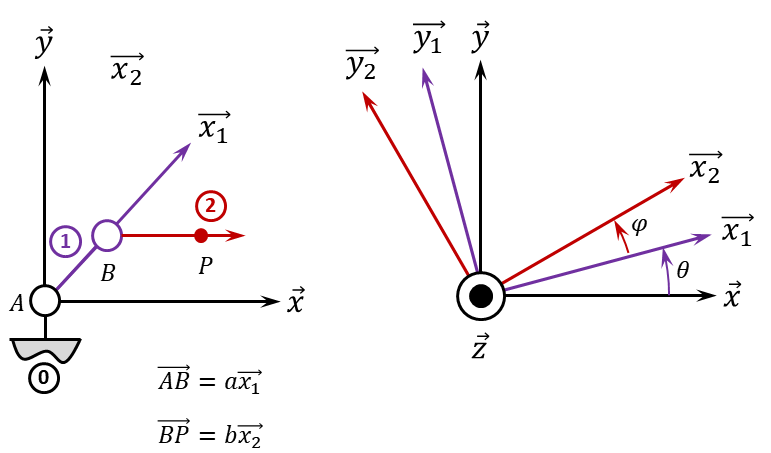
\includegraphics[width=\linewidth]{057_01}
\end{center}



\subparagraph{}
\textit{Exprimer les coordonnées du point $P$ en fonction de $\varphi$ et $\theta$.}
\ifprof
\begin{corrige}

\end{corrige}
\else
\fi



\subparagraph{}
\textit{Exprimer $\varphi$ et $\theta$ en fonction des autres paramètres (je ne sais pas si c'est possible).}
\ifprof
\begin{corrige}

\end{corrige}
\else
\fi


\subparagraph{}
\textit{Donner les valeurs angulaire de $\varphi$ et $\theta$ pour que le point $P$ suive une ligne droite du point $(L,-h)$ à $(L,h)$. NDLR : cette question ne me semble pas facile. Il faudra surement utiliser Python pour faire ces tracés. On pourra prendre $a=b=1$, $L=1$ et $h=1$.}
\ifprof
\begin{corrige}
\end{corrige}
\else
\fi
